\documentclass[11pt,a4paper]{article}
\usepackage[T1]{fontenc}
\usepackage[utf8]{inputenc}
\usepackage[french]{babel}
\usepackage{graphicx,booktabs,geometry,hyperref,caption,xcolor}
\geometry{margin=2.5cm}
\graphicspath{{../results/v_minimal/}{figures/}}
\hypersetup{colorlinks=true,linkcolor=blue,urlcolor=blue}

\title{Simulation d'une usine en V : premiers enseignements\\
\large Application de la Théorie des Contraintes (TOC) avec SimPy}
\author{Projet IndEng}
\date{\today}

\begin{document}
\maketitle

\begin{abstract}
Nous simulons une usine de type \textbf{V} (un flux amont partagé diverge vers
deux lignes produit) avec le moteur à événements discrets \texttt{indeng}
(SimPy). Vingt exécutions Monte-Carlo d'un scénario à demande variable
permettent d'identifier le goulot d'étranglement, de mesurer son impact sur les
délais et les retards, et d'illustrer les principes de la Théorie des
Contraintes : le débit de l'usine est dicté par sa ressource contrainte (CCR),
et non par la somme des capacités locales.
\end{abstract}

\section{Le modèle simulé}

L'usine en V comporte trois postes (figure~\ref{fig:topo}) :
\begin{itemize}
  \item \texttt{prep} (capacité 2) : poste amont partagé par les deux produits ;
  \item \texttt{line\_a} (capacité 1, temps 3) : produit \textbf{P1} ;
  \item \texttt{line\_b} (capacité 1, temps 6) : produit \textbf{P2}.
\end{itemize}

La demande est un processus de Poisson (taux 0,02 commande/unité de temps)
portant sur P1 ou P2, avec des quantités aléatoires entre 5 et 20. Les temps de
changement de série sont de 1 unité par défaut et de 3 unités lors d'un
changement de produit sur \texttt{prep}. L'ordonnancement est FIFO, l'horizon
de simulation est 2000 unités de temps, et chaque scénario est rejoué 20 fois
avec des graines différentes.

\begin{figure}[htbp]
  \centering
  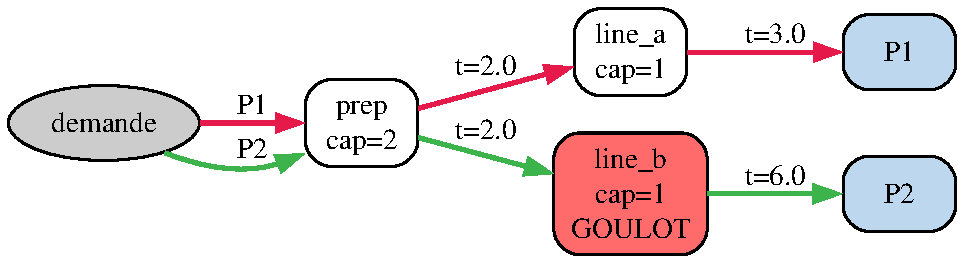
\includegraphics[width=0.85\textwidth]{topology_v.pdf}
  \caption{Topologie de l'usine en V (Graphviz). Le goulot \texttt{line\_b}
  est surligné en rouge. Les arêtes sont colorées par produit et étiquetées
  par le temps d'opération.}
  \label{fig:topo}
\end{figure}

\section{Résultats}

Le tableau~\ref{tab:kpis} regroupe les indicateurs clés (moyenne $\pm$ écart-type
sur 20 runs). Les figures~\ref{fig:util} à \ref{fig:prod} illustrent une
exécution représentative.

\begin{table}[htbp]
  \centering
  \caption{KPIs du scénario V (20 runs Monte-Carlo, horizon 2000).}
  \label{tab:kpis}
  \begin{tabular}{lrr}
    \toprule
    Indicateur & Moyenne & Écart-type \\
    \midrule
    Utilisation \texttt{prep} & 0,267 & 0,040 \\
    Utilisation \texttt{line\_a} & 0,375 & 0,094 \\
    Utilisation \texttt{line\_b} (goulot) & 0,668 & 0,147 \\
    Throughput P1 (unités) & 249,9 & 62,8 \\
    Throughput P2 (unités) & 222,8 & 48,9 \\
    Throughput total & 472,6 & 75,8 \\
    Lead time P1 & 80,5 & 10,5 \\
    Lead time P2 & 166,1 & 44,3 \\
    Makespan & 1959,8 & 31,6 \\
    Commandes terminées & 38,3 & 5,9 \\
    WIP moyen & 2,39 & 0,77 \\
    Commandes en retard & 8,5 & 5,3 \\
    Taux de retard & 21,4\,\% & 10,9\,\% \\
    \bottomrule
  \end{tabular}
\end{table}

\begin{figure}[htbp]
  \centering
  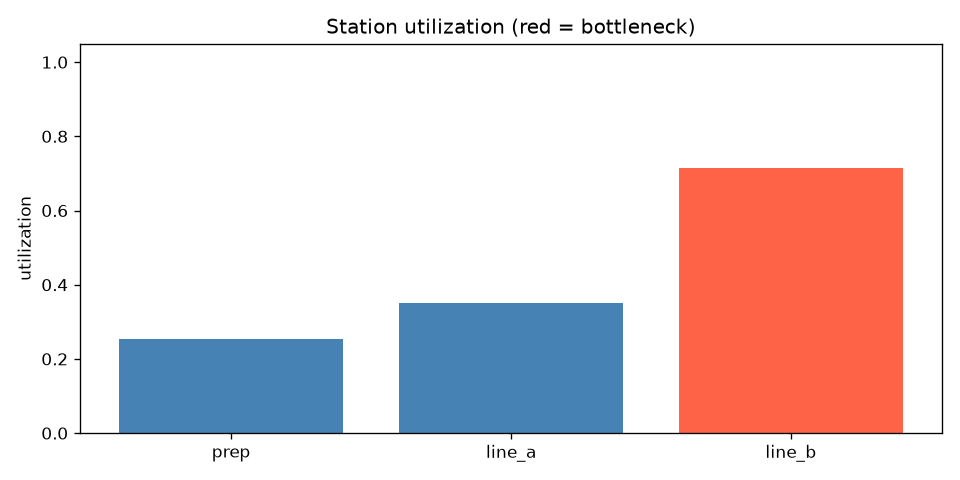
\includegraphics[width=0.7\textwidth]{utilization.png}
  \caption{Utilisation des postes : \texttt{line\_b} (rouge) est la ressource
  contrainte, nettement devant les autres.}
  \label{fig:util}
\end{figure}

\begin{figure}[htbp]
  \centering
  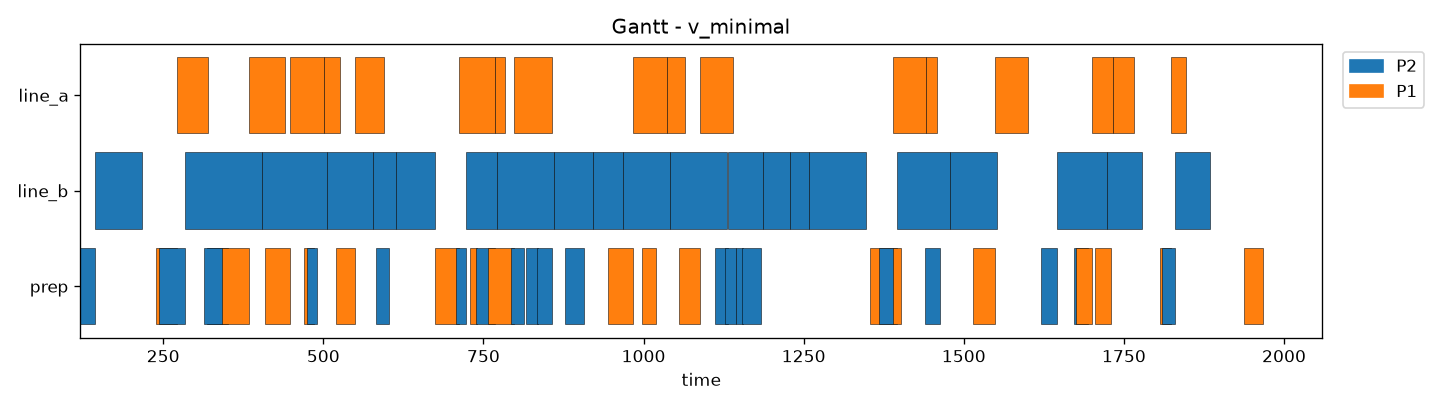
\includegraphics[width=0.95\textwidth]{gantt.png}
  \caption{Diagramme de Gantt d'un run : \texttt{prep} alterne les produits
  (setups), les lignes sont presque continûment occupées par leur produit.}
  \label{fig:gantt}
\end{figure}

\begin{figure}[htbp]
  \centering
  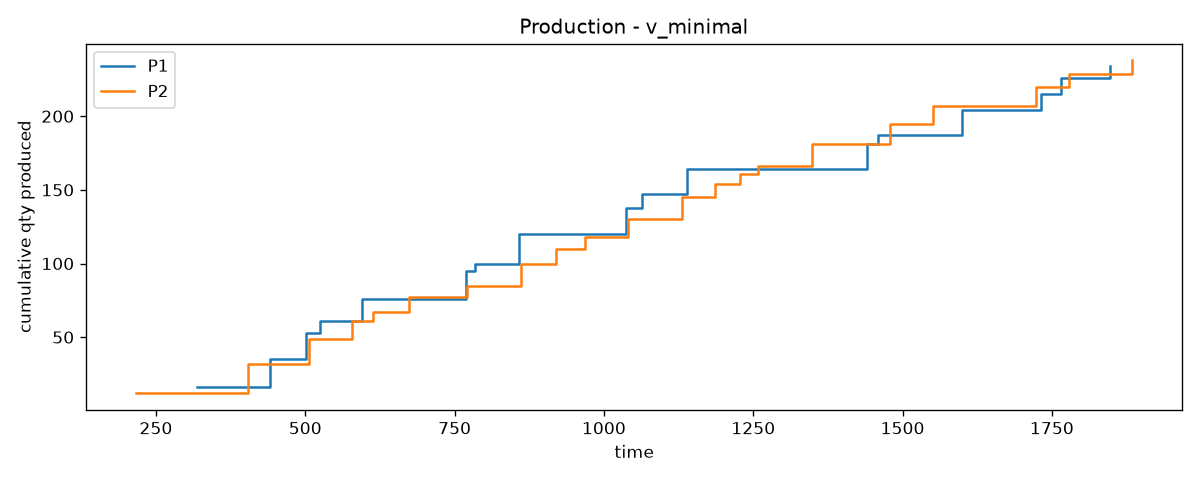
\includegraphics[width=0.85\textwidth]{production.png}
  \caption{Production cumulée de P1 et P2 : des pentes comparables, le débit
  étant cadencé par le goulot.}
  \label{fig:prod}
\end{figure}

\section{Que nous apprend cette simulation ?}

\subsection{Un seul poste dicte le débit de toute l'usine}
Le goulot \texttt{line\_b} est détecté comme poste le plus utilisé dans
19 runs sur 20 (utilisation 0,67 contre 0,27--0,38 pour les autres). C'est la
\emph{ressource contrainte} (CCR) au sens de la TOC : \textbf{le throughput de
l'usine est celui du goulot}, pas la somme des capacités des postes. Accélérer
\texttt{prep} ou \texttt{line\_a} n'augmenterait pas la production globale.

\subsection{Les files se forment devant le goulot, pas ailleurs}
Le lead time de P2 (166) est environ le double de celui de P1 (80) : les
commandes de P2 s'accumulent en amont de \texttt{line\_b}. Le diagramme de
Gantt montre d'ailleurs des lignes quasi pleines, signe d'un système tiré par
la contrainte. Le WIP moyen reste faible (2,4) : il n'y a pas d'en-cours
inutile qui s'accumule devant les postes non contraints.

\subsection{Sans buffer, la contrainte génère des retards}
Avec une échéance fixée à 2 fois le temps de passage nominal et aucun buffer
de temps devant le goulot, 21\,\% des commandes sont livrées en retard. C'est
le rôle du \textbf{Buffer} dans la méthode DBR (Drum-Buffer-Rope) : protéger le
goulot par un buffer de temps pour absorber la variabilité de la demande et
des postes amont.

\subsection{La variabilité impose le Monte-Carlo}
La demande étant aléatoire, les écarts-types sont élevés (throughput total :
$\pm$ 76 unités, taux de retard : $\pm$ 11 points). Une seule exécution ne
serait pas représentative : les 20 runs avec graines fixées donnent des
résultats reproductibles et des intervalles de confiance exploitables.

\subsection{Le levier d'amélioration est la contrainte elle-même}
Pour augmenter le débit de l'usine, la TOC prescrit d'\emph{élever la
contrainte} : réduire le temps de \texttt{line\_b} (6 $\to$ 3, ou capacité
2) aura un effet direct sur le throughput total et les retards, alors que
des gains sur \texttt{prep} n'en auraient quasiment pas (et créeraient du WIP
inutile).

\section{Limites et perspectives}

Ce premier modèle reste volontairement simple : une seule famille de produits
par ligne, pas de pannes ni de maintenance, des setups symétriques. Les
prochaines étapes du dépôt sont le scaffold des archétypes \textbf{A} et
\textbf{T} (figures~\ref{fig:topo-a} et~\ref{fig:topo-t}), la règle
d'ordonnancement \textbf{DBR} (scaffoldée dans \texttt{indeng/scheduling}), et
des buffers de temps configurables devant le goulot pour comparer les
politiques de protection.

\begin{figure}[htbp]
  \centering
  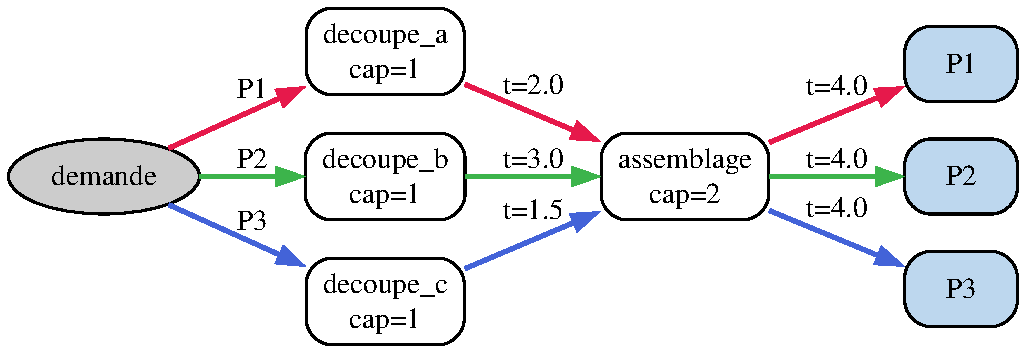
\includegraphics[width=0.8\textwidth]{topology_a.pdf}
  \caption{Archétype A (démonstration) : plusieurs composants convergent vers
  un assemblage.}
  \label{fig:topo-a}
\end{figure}

\begin{figure}[htbp]
  \centering
  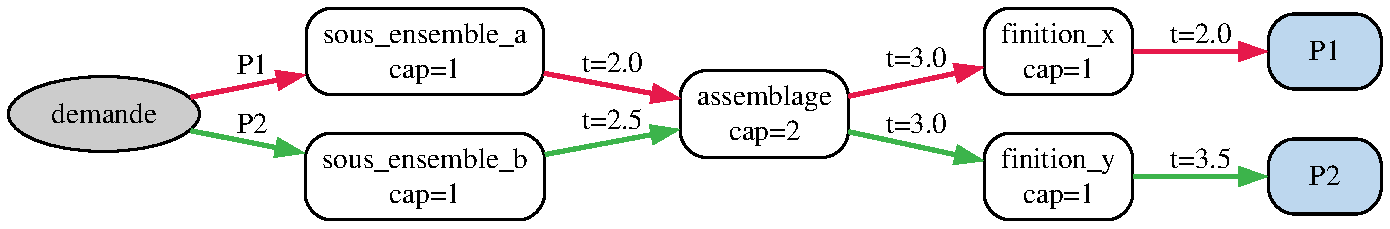
\includegraphics[width=0.95\textwidth]{topology_t.pdf}
  \caption{Archétype T (démonstration) : convergence vers l'assemblage puis
  divergence vers les finitions.}
  \label{fig:topo-t}
\end{figure}

\section{Reproductibilité}

\begin{verbatim}
pip install -e .
python -m indeng run config/scenarios/v_minimal.yaml --runs 20 --out out
python -m indeng graph config/scenarios/v_minimal.yaml --out out --highlight line_b
pytest   # 23 tests
\end{verbatim}

Les sorties versionnées (KPIs, événements, graphiques, topologies) sont dans
\texttt{results/}.

\end{document}
